\section{Begriffe und Elemente in Klassendiagrammen}

\subsection{Komposition}
Bei einer \textbf{Komposition} handelt es sich um eine \textit{Ganzes}-\textit{Teile}-Beziehung, bei der das \textit{Ganze} verantwortlich für die Erstellung und Beseitigung der \textit{Teile} ist.
Außerdem sind die \textit{Teile} an die \textbf{Existenz} des \textit{Ganzen} gebunden.\\
\textit{Teile} gehören immer zu \textit{genau einem} \textit{Ganzen}.\\
Eine Komposition wird dargestellt durch eine gefüllte Raute an der Klassenbox, die das \textit{Ganze} repräsentiert.\\

\noindent
Um sicherzustellen, dass ein Teil immer nur zu einem \textit{Ganzen} gehört, kann bspw. in einer Methode, die Informationen über ein Teil zurückliefert, eine Kopie des Teils zurückgegeben werden.
Dadurch ist sichergestellt, dass die Referenz auf ein existierendes Objekt nicht mehrfach verwendet werden kann.

\subsection{Aggregation}
Eine \textbf{Aggregation} ist in ihrer \semantischen Aussage unscharf (vgl.~\cite[40]{Buh09}).\\
Auch hier geht es um eine \textit{Ganzes}-\textit{Teile}-Beziehung, aber die \textit{Teile} können zu mehreren verschiedenen \textit{Ganzen} gehören.
Außerdem kann ein Teil dem \textit{Ganzen} jederzeit wieder entnommen werden und das \textit{Ganze} ist nicht verantwortlich für das Erstellen der \textit{Teile}, weshalb Implementierungen beim Hinzufügen von Teilen oft schon fertige Objekte erwarten, die jeweils eines der \textit{Teile} repräsentieren.

\subsection{Schnittstellen}
\textbf{Schnittstellen} geben eine Vertrag vor, den implementierende Klassen erfüllen:

\begin{itemize}
    \item eine Klasse, die die Schnittstelle implementiert, muss die deklarierten Operationen umsetzen
    \item eine einzelne Klasse kann beliebig viele Schnittstellen implementieren
    \item eine einzelne Schnittstelle kann von beliebig vielen Klassen implementiert werden
    \item Schnittstellen können andere Schnittstellen generalisieren
\end{itemize}

\noindent
Schnittstellen können mit dem Stereotyp \textcolor{blue}{\guillemotleft interface\guillemotright} über ihrem Namen in der Klassenbox gekennzeichnet werden.

\subsection{Abstrakte Klassen}
\textbf{Abstrakte Klassen} werden mit \code{{abstract}} gekennzeichnet\footnote{
``after or below its name`` (\cite[101]{OMG17})
}, oder der Klassenname wird \textit{kursiv} gesetzt.\\
Abstrakte Klassen können nicht instanziiert werden und können abstrakte Methoden und Methoden mit Implementierungen enthalten.\\
Hat eine Klasse eine abstrakte Methode, ist diese automatisch abstrakt.\\
Wird eine abstrakte Klasse abgeleitet, und die ableitende Klasse ist nicht abstrakt, müssen die abstrakten Methoden in der ableitenden Klasse implementiert werden.

\subsection{Assoziationsklasse (Attributierte Assoziation)}
Eine \textbf{Assoziationsklasse} erlaubt das Hinzufügen von Operationen und Attributen zu einer Assoziation (\cite[43]{Buh09}).

\blockquote[{\cite[277]{Oes05}}]{
Eine attributierte Assoziation ist immer dann nahe liegend, wenn Attribute oder Operationen gefunden werden, die weder der einen noch der anderen Klasse zugeordnet werden können, weil sie nämlich Eigenschaften der Beziehung selbst sind.
}.

\begin{tcolorbox}
Bei einer attributierten Assoziation dürfen zwei beteiligte Objekte maximal nur eine Beziehung zueinander haben (vgl.~\cite[277]{Oes05})\footnote{
\textit{Ostereich} führt dies ebenda auf Seite 278 weiter aus, in dem er beschreibt, wie eine attributierte Assoziation für ein \textit{Beschäftigtenverhältnis} zwischen \textit{Mitarbeiter} und \textit{Unternehmen} modelliert wird. Dabei wird davon ausgegangen, dass ein \textit{Mitarbeiter} nur über \textit{ein} Arbeitsverhältnis mit einem \textit{Unternehmen} in Beziehung stehen kann. Bestehen mehrere Arbeitsverhältnisse (\textit{Mitarbeiter} hat zu unterschiedlichen Zeitpunkten für das \textit{Unternehmen} gearbeitet), kann die attributierte Assoziation nicht verwendet werden.
}.
\end{tcolorbox}

\noindent
Wird eine attributierte Assoziation in eine gewöhnliche Assoziation transformiert, muss darauf geachtet werden, die Multiplizitäten richtig zu setzen (s. Abbildung~\ref{fig:assoziationsklasse}).

\begin{figure}
    \centering
    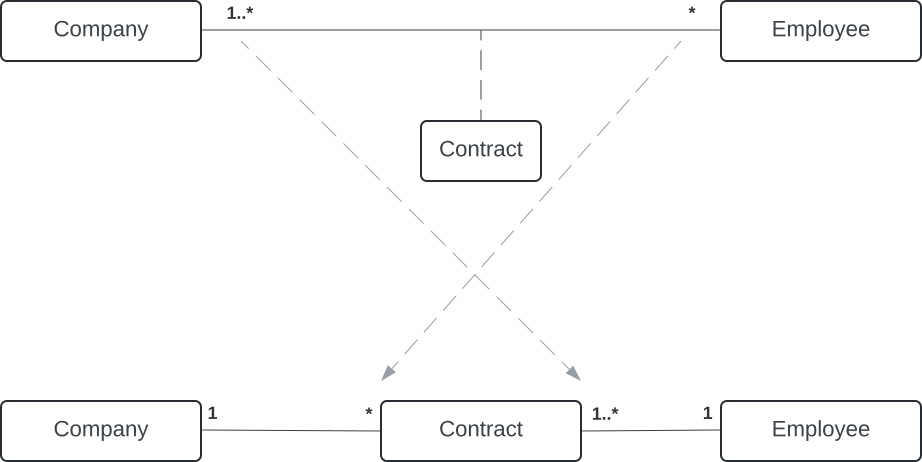
\includegraphics[scale=0.4]{part three/Klassendiagramme - Erweiterte Konzepte und Paketdiagramme/img/assoziationsklasse}
    \caption{Darstellung einer Assoziation mit Hilfe einer Assoziationsklasse (oben) sowie Transformation in gewöhnliche Assoziationen (unten). (Quelle: in Anlehnung an \cite[279, Abb. 4.4-11]{Oes05})}
    \label{fig:assoziationsklasse}
\end{figure}

\subsection{Templates (generische / parametrisierbare Klassen)}
Klassen, die als \textbf{Template} gekennzeichnet sind, stellen ``eine Beschreibung einer Klasse mit einem oder mehreren formalen Parametern`` (\cite[253]{Bal05})\footnote{
s.a. \cite[103 ff.]{OMG17}
} dar.\\

\noindent
Hierüber lassen sich bspw. Java-\texbf{Generics} modellieren.\\

\noindent
Eine Klasse wird zunächst mit einem Parameternamen gekennzeichnet.
Für einen konkreten Anwendungsfall wird dann eine Klasse als konkreter Parametertyp gebunden (s. Abbildung~\ref{fig:template} und nachfolgender Quelltext, beides nach \cite[81 f.]{Fow03b}).

\begin{minted}[mathescape,
    linenos,
    numbersep=5pt,
    gobble=2,
    fontsize=\small]{java}
    class RainbowBucket <T extends ValuableElement>{
    }

    RainbowBucket<Gold> potOfGolf;

\end{minted}
\begin{figure}
    \centering
    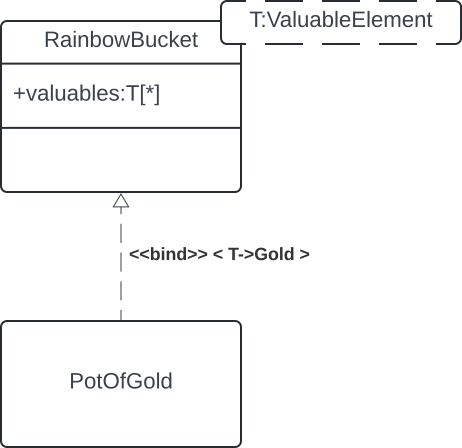
\includegraphics[scale=0.4]{part three/Klassendiagramme - Erweiterte Konzepte und Paketdiagramme/img/template}
    \caption{Parametrisierbare Klasse RainbowBucket. (Quelle: eigene)}
    \label{fig:template}
\end{figure}

\blockquote[{\cite[82, Hervorhebungen i.O.]{Fow03b}}]{
Using a derivation [Anm.: die Verwendung einer parametrisierbaren Klasse wie in Abbildung~\ref{fig:template} gezeigt] is \textit{not}
the same as subtyping, however. You are not allowed to add features to the bound element, which is completely specified by its template; you are adding only restricting type information. If you want to create features, you must create a subtype.
}